\chapter{Market microstructure models}
\label{chap:market_microstructure}
\section{Introduction}
The dominant framework utilized in financial market modeling is based on the condition of no arbitrage opportunities.
\begin{mydefinition}[Arbitrage]
	An arbitrage opportunity is present in a market when an economic actor can devise a
	trading strategy which is able to provide her a financial gain continuously, without initial
	investment, and without risk.
	\label{arbitrage}
\end{mydefinition}
In an efficient market, the exploitation of an arbitrage opportunity typically leads to its rapid elimination.\\
Considering fundamental analysis, Williams (1938), Graham and Dodd (1934) proposed thid definition of fundamental value:
\begin{mydefinition}[Fundamental values]
Intrinsic or Fundamental value of any security equals the discounted cash flow which that security gives title to, and actual price fluctuate around fundamental values, in formula:
\begin{equation}
	P_t = \sum_{k=0}^{\infty}\frac{1}{(1+r)^{k+1}} \expected{D_{t+k}}
\end{equation}
where $r$ is the constant discount rate and $D_t$ is the dividend payed at time $t$
\label{fundamental_price}
\end{mydefinition}
Working (1934) proposed that random walks generate patterns resembling stock prices, while Kendall (1953), Granger and Morgenstern (1963) conducted statistical analyses that revealed stock prices exhibit a random walk behavior.
\begin{myquote}
	If stock prices were patternless, was there any point to fundamental analysis? (LeRoy 1989)
\end{myquote}
When we say that two information sets $I$ and $J$ satisfy the condition $I \subset J$, it means that set $J$ contains more information or is more comprehensive than set $I$.\\`` In other words, $J$ is superior or more extensive in terms of information compared to $I$".
\begin{mydefinition}[Law of Iterated Expectations]
Given a random variable $X$:
\begin{equation}
	\expected{X | I} = \expected{\expected{X|J}|I}
\end{equation}
\end{mydefinition}
In simpler terms, if you have limited information denoted as $I$,the most accurate forecast you can make for a random variable $X$ is essentially the forecast you would make for $X$  if you had access to more comprehensive and superior information denoted as $J$.\\ In essence, having better information helps you make a more accurate prediction.\\
The law can be rewritten a:
\[
\expected{X - \expected{X|J}|I} = 0
\]
This implies that you cannot use limited information represented by $I$ to predict the forecast error that you would make if you had superior information denoted as $J$. Limited information doesn't allow you to account for the additional insights and knowledge that superior information would provide, making it impossible to accurately predict the forecast errors that would arise with better information.\\
Suppose that at a given time $t$, the price of a security, denoted as $P_t$, can be expressed as the rational expectation of a fundamental value $V$, taking into account the information available at that time, denoted as $I_t$:
\[
P_t = \expected{V | I_t} \equiv \expected{V}_t
\]
the expectation of the change over next period is:
\[
\expected{P_{t+1}-P_t}_t = \expected{\expected{V}_{t+1}-\expected{V}_{t}} = 0
\]
due to Law of Iterated Expectations. The actual changes in prices, when they occur, cannot be predicted using the information contained in the set $I_t$.
\begin{myquote}
A capital market is said to be efficient if it fully and correctly reects all relevant
information in determining security prices. Formally, the market is said to be efficient with respect to some information set if prices would be unaffected by revealing that information to all participants. Moreover, efficency with respect to an information set implies that it is impossible to make economic profits by trading on the basis of that information set.(Malkiel, 1992)
\end{myquote}
Informations doesn't change the price, surprise does it!
\begin{mydefinition}[Weak-form efficiency]
	The information set includes only the history of prices.
\end{mydefinition}
\begin{mydefinition}[Semistrong-form efficiency]
	The information set includes all the publicly available information.
\end{mydefinition}
\begin{mydefinition}[Strong-form efficiency:]
	The information set includes all information, i.e. also private information known to any market participant.
\end{mydefinition}
In the context of the Efficient Market Hypothesis, it follows that price fluctuations must be inherently unpredictable. In an increasingly efficient market, the sequence of price changes becomes more stochastic. The Random Walk Hypothesis is a commonly adopted model for prices, emphasizing market efficiency. It's important to note that the Random Walk Hypothesis imposes stricter limitations than the Martingale Hypothesis.
As we have seen in last chapter, the existence of autocorrelated returns, implies predictability using linear time series methods.
\begin{mysetting}[Roll Model]
\begin{itemize}
	\item Time is discrete and advances one unit any time a trade occurs
	\item All trades are conducted through a monopolistic dealer
	\item The efficient price follows a random walk
	\begin{equation}
	m_t = m_{t-1} + u_t
	\label{efficient_price_random}
	\end{equation}
	where $u_t$ is an independent identically distributed (i.i.d) noise with variance $\sigma^2_u$.
	\item At each time the dealer posts bid and ask prices.
	\item Dealer incurs a noninformational cost $c$ per trade (due to fixed costs: computers,telephone).No adverse selection and asymmetric information.
	\item The bid and the ask prices are:
	\[
	b_t - m_t -c \quad a_t = m_t + c
	\]
	and thus the spread is $2c$.
	\item The transaction price $p_t$:
	\begin{equation}
	p_t = m_t + q_tc
	\label{transaction_price}
	\end{equation}
where $q_t = +1(-1)$ if the customer is buyer (seller).
\end{itemize}
\end{mysetting}
\begin{mysetting}
	\begin{itemize}
\item Moreover $q_t$ are assumed serially independent and independent from prices ($m_t$ and
$p_t$ ). As we will see, this assumption is strongly violated in real data.
\end{itemize}
\end{mysetting}
Variance of transaction price increments is (remember: $q_{t-1}$ and $q_t$ are no correlated, $q_t,u_t$ are independent):
\[
\gamma_0 \equiv Var(\Delta p_t) = \expected{(p_t - p_{t-1})^2)} = \ldots = 2c^2 + \sigma_u^2
\]
That means: observed volatility is larger than the volatility of the efficient price!\\
The autocovariance of transaction price increments is:
\[
\gamma_1 \equiv Cov[\Delta p_{t-1} \Delta p_t] = -c^2
\]
and it is zero for lags larger than one. Thus observed returns are autocorrelated even if the efficient price is a martingale.\\
Empirical observations have revealed that the one-lag autocorrelation function of trade-by-trade return, and occasionally even in the context of high-frequency data like one-minute returns, exhibits a negative value. This phenomenon is commonly referred to as "bid-ask bounce".\\
Roll model was used to determine the spread from transaction data.\medskip \\
According to the Roll model, the volatility over $\tau$ consecutive trades is given by
\[
C(\tau) = \frac{\expected{(p_{t+\tau} - p_t})^2}{\tau} = \underbrace{\frac{\expected{(\sum_{t = 1}^{\tau} \Delta p_t)^2}}{\tau}}_{\textbf{diffusive process (random walk)}} = \sigma^2_u + \frac{2c^2}{\tau}
\]
Plot of $C(\tau)$ is called signature plot. More flat is plot, more diffusive is the process, more is random-walk.
\begin{center}
	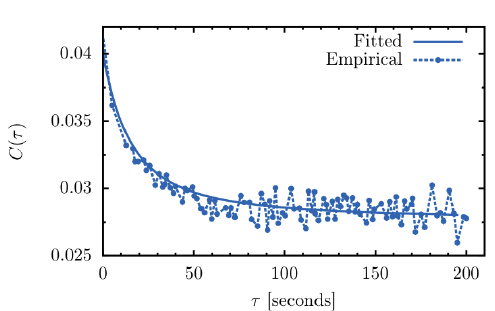
\includegraphics[width=0.5\textwidth]{picture/(2)signature_plot.png}
\end{center}
In the Roll model, the autocovariance pattern of transaction price increments is identical to that of a Moving Average (MA) process with a lag of 1 (MA(1)). It's important to note that the Roll model is essentially a structural model, but its time series representation can be seen as a statistical model.\\
\newpage
Assuming covariance stationarity allows us to apply the Wold theorem, which states that any zero-mean covariance stationary process $x_t$ can be represented as:
\[
x_t = \sum_{j=1}^{\infty} \theta_j\epsilon_{t-j} + \kappa_t
\]
where $\epsilon_t$ is a zero mean white noise process and $\kappa_t$ is a linearly deterministic process
(can be predicted arbitrarily well by a linear projection on past observation of $x_t$ ).\\
Structural models typically incorporate unobserved variables. For instance, in the original Roll model, neither $u_t$ nor $q_t$ are directly observable. Consequently, the efficient price mt remains unobserved as well, although estimating it would be of significant interest.\\
On the other hand, statistical models are well-suited for forecasting purposes. In the Roll model, one can directly observe $p_t$ and estimate $\gamma_0$ and $\gamma_1$ with relative ease.
In an MA(1) process, $x_t = \epsilon_t + \theta\epsilon_{t-1}$, they are related to the model's parameters as:
\[
\gamma_0 = (1 + \theta^2)\sigma_\epsilon^2 \qquad \gamma_1 = \theta\sigma_\epsilon^2 \qquad \sigma^2_{\epsilon} = Var[\epsilon_t] 
\]
If $|\theta| <1$, exixsts a convergent AR($\infty$) which is useful for forecasting.
\section{Asymmetric information models}

Asymmetric information models are designed to depict how informed traders interact with uninformed intermediaries, often in the presence of noise traders (these are necessary, they make market less efficient). In these models, the security's payoff typically exhibits a common value nature, with the primary benefit of owning the security being its resale value or terminal liquidating dividend, which is consistent for all holders.\\
However, for trading to occur, there must also be private value components. These are individual agents' needs for diversification or exposure to specific risks that are unique to each agent.\\
Initially, public information consists of shared knowledge about the probability structure of the economy. This includes information about the unconditional distribution of terminal security values and the distribution of agent types.\\
As the trading process unfolds, the most significant updates to the public information set come from market data, such as bids, asks, and the prices and volumes of trades. Consequently, the trading process involves transitioning from one well-defined information set to another, and it lacks properties like stationarity, ergodicity, and time-homogeneity. So that the market 'learns' from others, it expands its information set.\\
We hace 2 different models:
\begin{itemize}
	\item \textbf{Sequential trade models}: it involve traders arriving at the market one by one, randomly, independently, and individually. In a situation where an individual trader only engages in the market once, there is no necessity for them to consider the impact their actions might have on the subsequent decisions of other participants.
	\item \textbf{Strategic trader models:}  a single informed agent is capable of trading multiple times within the market (Kyle 1985). However, when a trader revisits the market for subsequent trades, they must engage in strategic calculations that take into account various factors. In both models, whether it's a single or repeat trade, each transaction discloses certain aspects of the trader's private information.
\end{itemize}
\subsection{Sequential model: Glosten and Milgrom (simplified)}
\begin{mysetting}[Sequential model: Glosten and Milgrom]
	\begin{itemize}
		\item One security with value (payoff) $V$ that is either low (\underline{$V$}) or high ($\overline{V}$). The probability of the low outcome is $\delta$ (indepentent from trading).
		\item The value is revealed after the market closes and it is not affected by trading.  It is determined by a random draw of nature before the market opens.
		\item Traders can be either informed (i.e. they know the value ($V$) outcome) or
		uninformed. The fraction of informed traders is $\mu$.
		\item A dealer posts bid and ask quotes, B and A.
		\item  He knows parameters (\underline{$V$}, $\overline{V}$, $\delta$, $\mu$)
		\item At each time step a trader is drawn at random from the population:
		\begin{itemize}
			\item If she is informed, she buys if $V = \overline{V}$ and sells if $V =$\underline{$V$}
			\item If she is informed, she buys and sells with equal probability.
		\end{itemize}
	   \item Transaction price is set by the dealer:
	   \begin{itemize}
	   	\item Buys(from traders) occur at dealer's ask price $A$
	   	\item Sells (from traders) occur at dealer's bid price $B$.
	   \end{itemize}
   \item The dealer does not know whether the trader is informed.
	\end{itemize}
\end{mysetting}
Let's rapresent probability tree:
	\begin{center}
		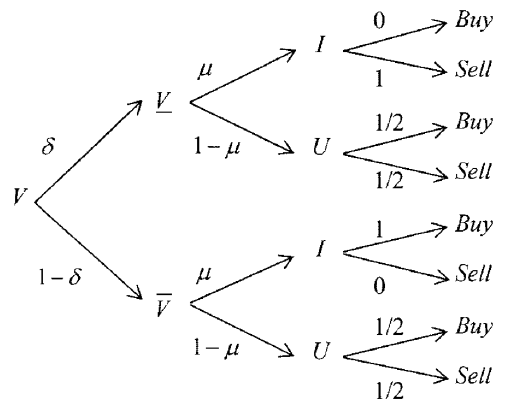
\includegraphics[width=0.5\textwidth]{picture/(3)prob_tree.png}
	\end{center}

Total probabilities are obtained by multiplication along the path ($U$=Uninformed, $I$=informed):
\begin{align*}
	&P(V = \text{\underline{$V$}}, U, \text{Buy}) = \delta (1 - \mu) \frac{1}{2}\\
	&P(\text{Buy}) = \frac{1 + \mu(1- 2 \delta)}{\delta}
\end{align*}

Let us consider the dealer:
\begin{itemize}
	\item The purchases and sales are not sensitive to quotes.
	\item If she is monopolist, she sets $A = \infty$  and $B = 0$
	\item Competition and regulation: "We assume that competition among dealers drive expected profit to zero".
\end{itemize}
The dealer uses Bayes rule to update her beliefs on $V$. Assume that the first trade is a buy, the updated value of her belief on $\delta$ is:
\[
\delta_1(\text{Buy}) = P (\text{\underline{$V$}}|\text{Buy}) = \frac{P(\text{\underline{$V$}},\text{Buy})}{P(\text{Buy})} = \frac{\delta(1 - \mu)}{1 + \mu(1-2\delta)}
\]
If the first is a sell, than her updated value of $\delta$ is:

\[
\delta_1(\text{Sell}) = P (\text{\underline{$V$}}|\text{Sell}) = \frac{P(\text{\underline{$V$}},\text{Sell})}{P(\text{Buy})} = \frac{\delta(1 + \mu)}{1 - \mu(1-2\delta)}
\]

Assume that the first trade is a buy. At the end of the day, the dealer's realized profit on the first transaction is $\Pi = A-V$(because it is a buy). Her exception of the profit is:
\[
\expected{\Pi|\text{Buy}} = A - \expected{V|\text{Buy}} = A - (\delta_1(\text{Buy}) \text{\underline{$V$}} + (1 - \delta_1(\text{Buy})\overline{V}))
\]
Due to competon, we impose $ \expected{\Pi|\text{Buy}} = 0$, than:

\[
A = \expected{V| \text{Buy}} = \frac{\text{\underline{$V$}} (1- \mu) \delta + \overline{V}(1 - \delta) (1 + \mu)}{1 + \mu(1- 2 \delta)}
\]
Analogues:
\[
B = \expected{V| \text{Sell}} = \frac{\text{\underline{$V$}} (1+ \mu) \delta + \overline{V}(1 - \delta) (1 - \mu)}{1 - \mu(1- 2 \delta)}
\]
Therefore the spread (before the first transaction) is set by the dealer at:
\[
A- B = \frac{4(1-\delta)\delta \mu (\overline{V} - \text{\underline{$V$}})}{1 - (1-2\delta)^2\mu^2}
\]
Simple case: $\delta = 1/2$:
\[
A-B = (\overline{V} - \text{\underline{$V$}})\mu
\]
The (initial) spread is proportional to the fraction of informed traders, the spread is a protection of the dealer to adverse selection from trading with informed traders.\medskip\\
Let us analysing the dynamics and let us see who loses money.\\
Assume that the first trade is a buy. From conditional expectation:
\[
\expected{V|\text{Buy}} = \expected{V|U,\text{Buy}}P(U|\text{Buy}) + \expected{V|I,\text{Buy}}P(I|\text{Buy})
\]
Using $A = \expected{V| \text{Buy}}$ and rearranging the terms:
\[
(A - \expected{V | U, \text{Buy}}) P (U|\text{Buy}) = - (A - \expected{V|I, \text{Buy}})P(I|\text{Buy})
\]
The left is dealer's gain from trading with the uninformed, the right hand is dealer's gain from trading with the informed. Wealth is transferred from uninformed to informed traders.\\
After the initial trade, the dealer updates her beliefs and update the quotes accordingly by using the expressions for the map from prior to posterior probabilities:
\[
\delta_k(\text{Buy}_k; \delta_{k-1}) = \frac{\delta_{k-1}(1 - \mu)}{1 + \mu(1-2\delta_{k-1})} \qquad \delta_k(\text{Sell}_k; \delta_{k-1}) = \frac{\delta_{k-1}(1 + \mu)}{1 - \mu(1-2\delta_{k-1})}
\]
We noticed thath:
\begin{itemize}
	\item Trade price is a martingale
	\item The spread declines over time and prices converges to the true value of $V$
	\item There is a price impact of prices, i.e., given a past history, a buy moves the price up and a sell moves the price down
\end{itemize}
\newpage
General comments about this model:
\begin{itemize}
	\item The Glosten Milgrom model makes the assumption that informed traders exclusively use market orders, which is not reflective of how trading typically occurs in limit order book markets.
	\item Nevertheless, this unrealistic assumption is employed for empirical purposes in estimating the probability of informed trading (known as PIN).
	\item The Glosten Milgrom model demonstrates that a significant portion of the spread is attributable to adverse selection, where informed traders exploit their information advantage.
	\item In classical microstructure analysis, the spread is typically decomposed into three components:
	\begin{itemize}
		\item Fixed noninformational cost (similar to the Roll model).
		\item Adverse selection cost (similar to the Glosten Milgrom model).
		\item Inventory cost (representing the spread that dealers apply to manage the risk associated with holding a large inventory).
	\end{itemize}	
\end{itemize}
\subsection{Strategic Model: Kyle}
The model addresses a scenario characterized by information asymmetry, the mechanism by which information influences prices, and the strategic decision-making of both the dealer and the informed trader. This model operates within an equilibrium framework.\\
It can take on several variations, including single-period, multi-period, and continuous-time settings. In this model, there are typically three key agents involved:
\begin{itemize}
	\item \textbf{Market Maker (MM) or Dealer}: This agent facilitates trading in the market.
	
	\item \textbf{Informed Trader}: This agent possesses private information that can impact trading decisions.
	
	\item \textbf{Noise Traders}: These are numerous traders who engage in the market without possessing any significant private information, and their trading behavior is often driven by random or non-informative factors.
\end{itemize}
\begin{mysetting}[Strategic model:Kyle (one period)]
	\begin{itemize}
		\item The terminal (liquidation) value $v$ of an asset is normally distributed with mean $p0$ and variance $\Sigma_0$.
		\item The informed trader knows $v$ and enters a demand $x$ (volume).
		\item Noise traders submit a net order flow $u$, which is Gaussian distributed with mean zero and variance $\sigma_u^2$
	\end{itemize}
\end{mysetting}
\begin{mysetting}
		\begin{itemize}
			\item $x$ and $u$ are signed order flows, i.e. they are the purchased volume if positive, and
			the sold volume if negative.
			\item The MM observes the total demand $y = x + u$ and then sets a price $p$. All the trades are cleared at $p$, any imbalance is exchanged by the MM.   
			\item  However the MM knows that there is an informed trader and if the total demand is
			large (in absolute value) she is likely to incur in a loss. Thus the MM protects
			herself by setting a price that is increasing in the net order flow.
			\item The solution to the model is an expression of this trade-off
    \end{itemize}
\end{mysetting}
Let us analsing informed trader setting. She conjectures that the MM uses a linear price adjustment rule $p = \lambda y + \mu$, where $\lambda$ is inversely related to liquidity. Her profit is:
\[
\pi = (v-p)x = x[v - \lambda(u+x) - \mu])
\]
with expected profit:
\[
\expected{\pi} = x(v - \lambda x - \mu)
\]
It is a parabola, the traders maximizes it if:
\[
x = \frac{v - \mu}{2\lambda}
\]
In Kyle's model the informed trader can loose money, but on average she makes profit.\medskip \\
Let us analsing informed MM. Under the hypotesis that trader's demand is linear in $v$: $x = \alpha + \beta v$. So that MM knows optimizazion problem, $MM$ solves:
\[
\frac{v - \mu}{2\lambda} = \alpha + \beta v
\]
Solving it (similarity method) gives:
\[
\alpha = -\frac{\mu}{2\lambda} \qquad \beta = \frac{1}{2\lambda}
\]
As liquidity drops, the informed agent trade less, so MM observes $y$ and sets:
\[
p = \expected{v|y}
\]
In order to solve it, the following property is useful:
\newpage
\begin{mytheorem}[Expected value normal variables]
	If $X$ and $Y$ are bivariate normal variables:
	\[
	\expected{Y|X=x} = \mu_Y + \frac{\sigma_{XY}}{\sigma^2_X}(x - \mu_x)
	\]
	$\mu_i$ is the mean, $\sigma_{XY}$ is covariance, $\sigma_X$ variance.
\end{mytheorem}
we find:
\[
\expected{v|y}= \expected{v| u + \alpha + \beta v}
\]
solution is:
\[
\alpha = -p_0\sqrt{\frac{\sigma_u^2}{\Sigma_0}} \qquad \mu = p_0 \qquad \lambda = \frac{1}{2}\sqrt{\frac{\Sigma_0}{\sigma_u^2}} \qquad \beta = \sqrt{\frac{\sigma_u^2}{\Sigma_0}}
\]
substitute this coefficient in price formula, we obtain:
\begin{equation}
	p = p_0 + \frac{1}{2}\sqrt{\frac{\Sigma_0}{\sigma_u^2}}y
	\label{Kyle price}
\end{equation}
we notice:
\begin{itemize}
	\item more noise traders imply more liquidity market.
	\item $p-p_0 \propto y$, smaller $\lambda$ means a more liquidity market.
	\item Informed trader trade more if her hide between noise
	\item Informed trader take profit from noise traders.
	\item noise traders loose money and MM breaks even
\end{itemize}
Informed agent volume is:
\[
x = (v-p_0)\sqrt{\frac{\sigma_u^2}{\Sigma_0}} \Rightarrow \expected{\pi} = \frac{(v - p_0)^2}{2}\sqrt{\frac{\sigma_u^2}{\Sigma_0}}
\]
\begin{mysetting}[Strategic model:Kyle (multiple period)]
	\begin{itemize}
		\item There are $N$ auctions, each taking place at time $0=t_0<\ldots<t_N=1$
		\item The liquidation value of the asset is $v$, normally distributed with mean $p_0$ and
		variance $\Sigma_0$
		\item The quantity traded by noise traders in auction $n$ is $\Delta u_n = u_n - u_{n-1}$, where $u_n$ is a Brownian motion with zero mean and instantaneous variance $\sigma^2_u$
		\item $x_n$ is the aggregate position of the informed after the $n$th auction and $\Delta x_n = x_n - x_{n-1}$ is the quantity traded in this auction
	\end{itemize}
\end{mysetting}
\begin{mysetting}
	\begin{itemize}
				\item Each auction is divided in two steps:
		\begin{itemize}
			\item The informed and the noise traders place the aggregate demand $y = \Delta x_n + \Delta u_n$
			\item The market maker sets the liquidation price $p_n$
		\end{itemize}
	\end{itemize}
\end{mysetting}
The informed trader's trading strategy is a vector of functions $X = \langle X_1,\ldots,X_N \rangle$, where:
\[
x_n = X_n(p_1,\ldots,p_{n-1},v)
\]
while market maker pricing rule is a vector of function $P = \langle P_1,\ldots,P_N \rangle$, where:
\[
p_n = P_n(x_1+u_1,\ldots,x_n+u_n)
\]
The profit of the informed on position acquired at auctions $n,\ldots,N$ is:
\[
\pi_n = \sum_{k=n}^{N} (v-p_k)x_k
\]
A sequential auction equilibrium is a pair $X,P$ such that:
\begin{itemize}
	\item Profit maximization: $\forall n =1,\ldots,N$ and $\forall X'$ s.t. $X'_1 =X_1,\ldots,X'_{n-1} = X_{n-1}$ it is:
	\[
	\expected{\pi_n(X,P)|p_1,\ldots,p_{n-1},v} \geq \expected{\pi_n(X',P)|p_1,\ldots,p_{n-1},v}
	\]
	\item Market efficiency: $\forall n = 1,\ldots,N$ it is:
	\[
	p_n = \expected{v|x_1 + u_1,\ldots, x_n + u_n}
	\]
\end{itemize}
A linear equilibrium is a sequential auction equilibrium in which the functions $X$ and $P$ are linear, recursive linear equilibrium is a linear equilibrium such that, given $\exists \lambda_1,\ldots, \lambda_N, \ \forall n = 1,\ldots,N$:
\begin{equation}
	p_n = p_{n-1} + \lambda_n(\Delta x_n + \Delta u_n)
\end{equation}
\newpage
\begin{mytheorem}[Equilibrium Linear equilibrium Kyle Model multiple periods]
	Exist a unique linear equilibrium and this equilibrium is a recursive linear equilibrium. This equilibrium is given by:
	\begin{align*}
		&\Delta x_n = \beta_n(v - p_{n-1}) \Delta t_n \\
		&\Delta p_n = \lambda_n(\Delta x_n + \Delta u_n) \\
		& \Sigma_n \equiv var[v| \Delta x_1 + \Delta u_1,\ldots,\Delta x_n + \Delta u_n] = (1- \beta_n \lambda_n \Delta t_n)\Sigma_{n-1}\\
		& \expected{\pi_n|p_1,\ldots,p_{n-1},v} = \alpha_{n-1}(v - p_{n-1})^2 + \delta_{n-1}
	\end{align*}
coefficient are:
\begin{align*}
	& \alpha_{n-1} = \frac{1}{4 \lambda_n (1 - \alpha_n \lambda_n)}\\
	& \delta_{n-1} = \delta_n + \alpha_n \lambda^2_n \sigma^2_u \Delta t_n \\
	& \beta_n \Delta t_n = \frac{1 - 2\alpha_n \lambda_n}{2 \lambda_n (1 - \alpha_n \lambda_n)} \\
	& \lambda_n = \beta_n \Sigma_n / \sigma^2_u \\
	& \Sigma_n = (1 - \beta_n\lambda_n\Delta t_n)\Sigma_{n-1}
\end{align*}
Given final condition: $\alpha_n = 0, \delta_n = 0, \lambda_n(1-\alpha_n\lambda_n)>0$
\end{mytheorem}
\begin{mytheorem}[Equilibrium Kyle model in continuous time ($N \to \infty$)]
In continuous time, the equation for profit, informed order flow and price are:
\begin{align*}
	& d\pi(t) = [v-p(t)]dx(t) \\
	& dx(t) = \beta(t)[v - p(t)]dt\\
	& dp(t) = \lambda(t)[dx(t) + du(t)]
\end{align*}
In the recursive continuous auction equilibrium, if the trading takes place in $t \in [0,1]$, that is:
\begin{align*}
	&\lambda(t) = \sqrt{\Sigma_0 / \sigma_u^2} \\
	& \Sigma(t) = (1-t)\Sigma_0 \\
	& \beta(t) = \sigma_u \Sigma_0^{-1/2} / (1-t)\\
	& \alpha(t) = \frac{1}{2}\sqrt{\sigma_u^2/ \Sigma_0}\\
	& \delta(t) = \frac{1}{2}\sqrt{\sigma_u^2\Sigma_0}(1-t)
\end{align*}
\end{mytheorem}
\newpage
General comments on Kyle model:
\begin{itemize}
	\item The informed agent splits her order flow in order to hide in the noise trader order flow
	\item Linear price impact
	\item Uncorrelated total order flow
	\item Permanent and fixed impact
	\item Cariance of fundamental value $v$ declines
\end{itemize}
\subsection{Market impact}
There are different definition of price impact:
\begin{itemize}
	\item Impact of an individual market order of size $v$
	\item The correlation of the average price change in a given time interval $T$ with the total
	market order imbalance in the same interval (i.e. the sum of the signed volume $\pm v$ of all individual trades.)
	\item Cross impact, i.e. how do trades on asset A impact the price of asset B (important for portfolio).
	\item The impact of a given order of size $Q$, executed with many trades in a given direction, originating from the same agent.
\end{itemize}
During the course of the discussion, we will call Large order executed as: Metaorders.\\
For Kyle model, the average price variation due to a signed volume $\epsilon v$ is:
\[
\Delta p = \lambda \epsilon v
\]
$\lambda$ is the inverse of liquidity and $\epsilon$ is $\pm 1$ if it is buyer(seller).\\ We can show that:
\begin{itemize}
	\item the impact of single order is linear in volume and permanent:
	\[
	R_{\text{so}}(T) = \expected{(p_T - p_0)\cdot \epsilon_0} = \lambda \expected{v}
	\]
	\item the impact of aggregated order flow is linear in the volume imbalance:
	\[
	p_T = p_0 + \lambda \sum_{n=0}^{N-1} \epsilon_nv_n + \sum_{n = 0}^{N-1} \eta_n
	\]
	\item The price impact of metaorder of total volume $Q$ is linear:
	\[
	R_{\text{mo}}(T|Q) = \expected{(p_T - p_0) \cdot \epsilon_{\text{mo}}| \sum_{n \in \text{mo} = Q}} = \lambda Q
	\]
	\item time correlation properties of returns are 'inherited' by order flow
\end{itemize}
\newpage
Empirical data shows a sublinear (concave) volume dependence of impact of individual orders:
\[
\expected{\Delta p|v} \equiv R_{\text{so}}(T =1 |v) \propto v^{\psi}; \qquad \psi \in[0.1,0.3]
\]
or even a logarithmic dependence:
\[
R_{\text{so}}(T = 1|v)\propto \ln v
\]
that is in contrast with Kyle prediction.
\begin{mydefinition}[Market impact]
	The expected average price change between beginning and end of a metaorder of size $Q$, empirically fit by:
	\begin{equation}
		\Delta \ln p \equiv \mathcal{I}(Q) = \pm Y \sigma_d \left(\frac{Q}{V_D}\right)^\delta
	\end{equation}
where $\sigma_D$ is daily volatily, $V_D$ daily volume traded, $\pm$ if buy(sell), $\delta \sim 1/2$ 
\end{mydefinition}
There is a weakness in this formula, it is temporally independent.
\subsection{Market order flow and Autocorrelation function}
In this context, our attention is directed towards orders that initiate transactions, specifically market orders. A buy market order tends to increase the price, while a sell market order tends to decrease it (on average). The flow of market orders is a reflection of the supply and demand for shares in the market.
A market order is defined by two key attributes: a volume denoted as $v$ and a sign, represented as $\epsilon = 1$ if buy, $-1$ if sell.\\
We are examining the time series in terms of market order time, which means that time progresses by one unit each time a new market order is placed.\\
Sample autocorrelation function of sign is:
\[
C(\tau) = \frac{1}{N} \sum_t \epsilon_t\epsilon_{t +\tau} - \left(\frac{1}{N} \sum_t \epsilon_t\right)^2
\]
where $N$ is the length of the time series.
\begin{center}
	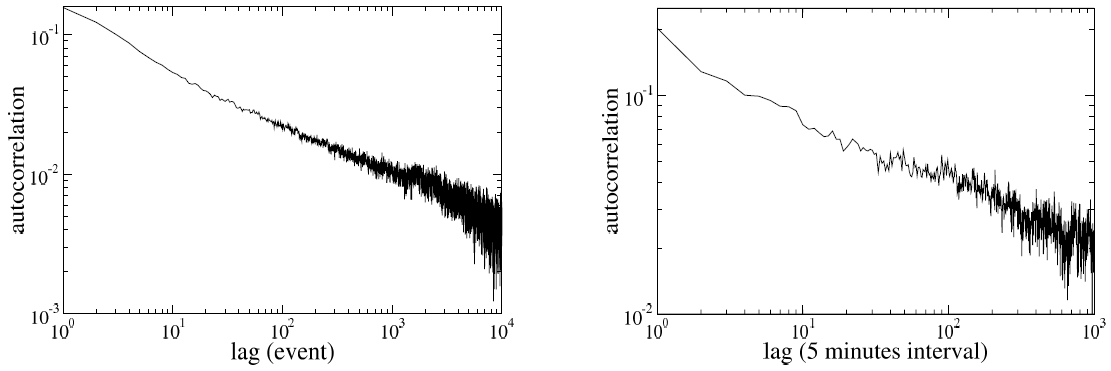
\includegraphics[width=0.5\textwidth]{picture/(4)autocorr_order_flow.png}
\end{center}
Asymptotically autcorrelation decays as:
\[
C(\tau) \sim \tau^{-\gamma} = \tau^{2H-2}
\]
$H$ is called Hurst exponent and it is $H \simeq 0.75$
\begin{mydefinition}[Long memory process]
Let $\gamma(k)$ be the autocovariance function of a time series $X_t$, a process is long memory if in the time $k \to \infty$ it is:
\[
\gamma(k) \sim k^{-\gamma} L(k) \qquad \gamma \in (0,1)
\]
where $L(k)$ is slowly varying function
\end{mydefinition}
Hurst exponent is defined as $H = 1- \gamma /2$\\
We can also provide a definition in the frequency domain.
\begin{mydefinition}[Long memory process (frequency)]
In long memory process, the spectral density diverges for low frequencies $\omega \to 0$ as:
\[
g(\omega) \simeq \omega^{1- 2H} L(\omega)
\]
\end{mydefinition}
The integrated process is super diffusive: $Var(\sum_{s=0}^{t} X_s) \sim t^{2H}$.\\
So that $H >1/2$, process grows really fast (remember, in random walk $Var(X) \sim t$) .\\
An example is fractional ARIMA (fARIMA) or fractional Brownian motion:
\[
(1-L)^d X_t = \epsilon_t \qquad d = H - 1/2
\]
Two proposed explanations have emerged for the origin of long-memory in order flow:
\begin{itemize}
\item Herding Among Market Participants (LeBaron and Yamamoto, 2007): Agents tend to exhibit herding behavior either because they are responding to the same signals or because they imitate each other's trading strategies. This interaction can be both direct and indirect.

\item Order Splitting (Lillo, Mike, and Farmer, 2005): To prevent the disclosure of their true intentions, large investors fragment their trades into smaller pieces and execute them incrementally, a concept originally introduced by Kyle in 1985. This practice converts the heavy tail of large order volume distributions into correlated order flow.
\end{itemize}
Is it feasible to empirically measure the contributions of herding and order splitting to the autocorrelation observed in order flow? It's worth noting that this inquiry is part of the broader question regarding the origin of the diagonal effect as raised in the work of Biais, Hillion, and Spatt in 1995.\\
Assuming that we know the identity of the investor placing any market order, for each investor $i$ we define a time series of market order sign $\epsilon_t^i$ which is equal to zero if the market order at time $t$ was not placed by investor $i$ and equal to the market order sign otherwise.\\
Under this condition, autocorrelation can be rewritten as:
\[
C(\tau) = \frac{1}{N} \sum_t \sum_{i,j} \epsilon^i_t \epsilon^j_{t + \tau} - \left(\frac{1}{N} \sum_t \sum_i \epsilon^i_t\right)^2
\]
We can rewrrite it as $C(\tau) = C_{\text{split}}(\tau) + C_{\text{herd}}(\tau)$, where:
\begin{align*}
	& C_{\text{split}}(\tau) = \sum_i \left(\sum_i P^{ii}(\tau) \left[ \frac{1}{N^{ii}(\tau)} \sum_t \epsilon_t^i\epsilon^i_{t+\tau}\right]- \left[P^i \frac{1}{N^i} \sum_t \epsilon^i_t\right]^2\right)\\
	& C_{\text{heard}}(\tau) = \sum_{i\neq j} \left(\sum_i P^{ij}(\tau) \left[ \frac{1}{N^{ij}(\tau)} \sum_t \epsilon_t^i\epsilon^j_{t+\tau}\right]- P^iP^j\left[ \frac{1}{N^i} \sum_t \epsilon^i_t\right]\left[ \frac{1}{N^j} \sum_t \epsilon^j_t\right]\right)
\end{align*}
$N^i$ is the number of market orders placed by agent $i$, $P^i = N^i/N$ (probability agent $i$ take ordet at time $t$), $N^{ij}(\tau)$ is the number of time that an order from investor $i$ at time $t$ is followed by an order from investor $j$ at time $t + \tau$ and $P^{ij}(\tau) = N^{ij}(\tau)/N$.\\
Empirically, hear decomposition is bigger.
\begin{center}
	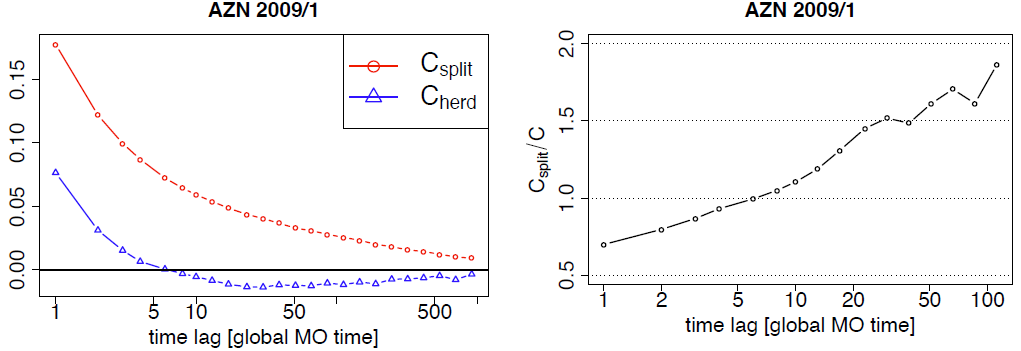
\includegraphics[width=0.6\textwidth]{picture/(5)autocorr_herd.png}
\end{center}